% Options for packages loaded elsewhere
% Options for packages loaded elsewhere
\PassOptionsToPackage{unicode}{hyperref}
\PassOptionsToPackage{hyphens}{url}
\PassOptionsToPackage{dvipsnames,svgnames,x11names}{xcolor}
%
\documentclass[
  letterpaper,
  DIV=11,
  numbers=noendperiod]{scrartcl}
\usepackage{xcolor}
\usepackage{amsmath,amssymb}
\setcounter{secnumdepth}{5}
\usepackage{iftex}
\ifPDFTeX
  \usepackage[T1]{fontenc}
  \usepackage[utf8]{inputenc}
  \usepackage{textcomp} % provide euro and other symbols
\else % if luatex or xetex
  \usepackage{unicode-math} % this also loads fontspec
  \defaultfontfeatures{Scale=MatchLowercase}
  \defaultfontfeatures[\rmfamily]{Ligatures=TeX,Scale=1}
\fi
\usepackage{lmodern}
\ifPDFTeX\else
  % xetex/luatex font selection
\fi
% Use upquote if available, for straight quotes in verbatim environments
\IfFileExists{upquote.sty}{\usepackage{upquote}}{}
\IfFileExists{microtype.sty}{% use microtype if available
  \usepackage[]{microtype}
  \UseMicrotypeSet[protrusion]{basicmath} % disable protrusion for tt fonts
}{}
\makeatletter
\@ifundefined{KOMAClassName}{% if non-KOMA class
  \IfFileExists{parskip.sty}{%
    \usepackage{parskip}
  }{% else
    \setlength{\parindent}{0pt}
    \setlength{\parskip}{6pt plus 2pt minus 1pt}}
}{% if KOMA class
  \KOMAoptions{parskip=half}}
\makeatother
% Make \paragraph and \subparagraph free-standing
\makeatletter
\ifx\paragraph\undefined\else
  \let\oldparagraph\paragraph
  \renewcommand{\paragraph}{
    \@ifstar
      \xxxParagraphStar
      \xxxParagraphNoStar
  }
  \newcommand{\xxxParagraphStar}[1]{\oldparagraph*{#1}\mbox{}}
  \newcommand{\xxxParagraphNoStar}[1]{\oldparagraph{#1}\mbox{}}
\fi
\ifx\subparagraph\undefined\else
  \let\oldsubparagraph\subparagraph
  \renewcommand{\subparagraph}{
    \@ifstar
      \xxxSubParagraphStar
      \xxxSubParagraphNoStar
  }
  \newcommand{\xxxSubParagraphStar}[1]{\oldsubparagraph*{#1}\mbox{}}
  \newcommand{\xxxSubParagraphNoStar}[1]{\oldsubparagraph{#1}\mbox{}}
\fi
\makeatother


\usepackage{longtable,booktabs,array}
\usepackage{calc} % for calculating minipage widths
% Correct order of tables after \paragraph or \subparagraph
\usepackage{etoolbox}
\makeatletter
\patchcmd\longtable{\par}{\if@noskipsec\mbox{}\fi\par}{}{}
\makeatother
% Allow footnotes in longtable head/foot
\IfFileExists{footnotehyper.sty}{\usepackage{footnotehyper}}{\usepackage{footnote}}
\makesavenoteenv{longtable}
\usepackage{graphicx}
\makeatletter
\newsavebox\pandoc@box
\newcommand*\pandocbounded[1]{% scales image to fit in text height/width
  \sbox\pandoc@box{#1}%
  \Gscale@div\@tempa{\textheight}{\dimexpr\ht\pandoc@box+\dp\pandoc@box\relax}%
  \Gscale@div\@tempb{\linewidth}{\wd\pandoc@box}%
  \ifdim\@tempb\p@<\@tempa\p@\let\@tempa\@tempb\fi% select the smaller of both
  \ifdim\@tempa\p@<\p@\scalebox{\@tempa}{\usebox\pandoc@box}%
  \else\usebox{\pandoc@box}%
  \fi%
}
% Set default figure placement to htbp
\def\fps@figure{htbp}
\makeatother


% definitions for citeproc citations
\NewDocumentCommand\citeproctext{}{}
\NewDocumentCommand\citeproc{mm}{%
  \begingroup\def\citeproctext{#2}\cite{#1}\endgroup}
\makeatletter
 % allow citations to break across lines
 \let\@cite@ofmt\@firstofone
 % avoid brackets around text for \cite:
 \def\@biblabel#1{}
 \def\@cite#1#2{{#1\if@tempswa , #2\fi}}
\makeatother
\newlength{\cslhangindent}
\setlength{\cslhangindent}{1.5em}
\newlength{\csllabelwidth}
\setlength{\csllabelwidth}{3em}
\newenvironment{CSLReferences}[2] % #1 hanging-indent, #2 entry-spacing
 {\begin{list}{}{%
  \setlength{\itemindent}{0pt}
  \setlength{\leftmargin}{0pt}
  \setlength{\parsep}{0pt}
  % turn on hanging indent if param 1 is 1
  \ifodd #1
   \setlength{\leftmargin}{\cslhangindent}
   \setlength{\itemindent}{-1\cslhangindent}
  \fi
  % set entry spacing
  \setlength{\itemsep}{#2\baselineskip}}}
 {\end{list}}
\usepackage{calc}
\newcommand{\CSLBlock}[1]{\hfill\break\parbox[t]{\linewidth}{\strut\ignorespaces#1\strut}}
\newcommand{\CSLLeftMargin}[1]{\parbox[t]{\csllabelwidth}{\strut#1\strut}}
\newcommand{\CSLRightInline}[1]{\parbox[t]{\linewidth - \csllabelwidth}{\strut#1\strut}}
\newcommand{\CSLIndent}[1]{\hspace{\cslhangindent}#1}



\setlength{\emergencystretch}{3em} % prevent overfull lines

\providecommand{\tightlist}{%
  \setlength{\itemsep}{0pt}\setlength{\parskip}{0pt}}



 


\usepackage{booktabs}
\usepackage{caption}
\usepackage{longtable}
\usepackage{colortbl}
\usepackage{array}
\usepackage{anyfontsize}
\usepackage{multirow}
\KOMAoption{captions}{tableheading}
\makeatletter
\@ifpackageloaded{caption}{}{\usepackage{caption}}
\AtBeginDocument{%
\ifdefined\contentsname
  \renewcommand*\contentsname{Table of contents}
\else
  \newcommand\contentsname{Table of contents}
\fi
\ifdefined\listfigurename
  \renewcommand*\listfigurename{List of Figures}
\else
  \newcommand\listfigurename{List of Figures}
\fi
\ifdefined\listtablename
  \renewcommand*\listtablename{List of Tables}
\else
  \newcommand\listtablename{List of Tables}
\fi
\ifdefined\figurename
  \renewcommand*\figurename{Figure}
\else
  \newcommand\figurename{Figure}
\fi
\ifdefined\tablename
  \renewcommand*\tablename{Table}
\else
  \newcommand\tablename{Table}
\fi
}
\@ifpackageloaded{float}{}{\usepackage{float}}
\floatstyle{ruled}
\@ifundefined{c@chapter}{\newfloat{codelisting}{h}{lop}}{\newfloat{codelisting}{h}{lop}[chapter]}
\floatname{codelisting}{Listing}
\newcommand*\listoflistings{\listof{codelisting}{List of Listings}}
\makeatother
\makeatletter
\makeatother
\makeatletter
\@ifpackageloaded{caption}{}{\usepackage{caption}}
\@ifpackageloaded{subcaption}{}{\usepackage{subcaption}}
\makeatother
\usepackage{bookmark}
\IfFileExists{xurl.sty}{\usepackage{xurl}}{} % add URL line breaks if available
\urlstyle{same}
\hypersetup{
  pdftitle={Clinical Trial On Pleural Cavity Opening During Median Sternotomy},
  pdfauthor={Rafik Margaryan, MD, PhD; Giacomo Bianchi, MD, PhD},
  pdfkeywords={Clinical Trial, Cardiac Surgery},
  colorlinks=true,
  linkcolor={blue},
  filecolor={Maroon},
  citecolor={Blue},
  urlcolor={Blue},
  pdfcreator={LaTeX via pandoc}}


\title{Clinical Trial On Pleural Cavity Opening During Median
Sternotomy}
\author{Rafik Margaryan, MD, PhD \and Giacomo Bianchi, MD, PhD}
\date{2025-04-13}
\begin{document}
\maketitle
\begin{abstract}
Clinicsl Trials are the backbone of the modern medicine. They are the
only way to test securly a hypothesis and to put out an evidence based
medicine. In this paper we will discuss the first and second stage of a
clinical trial on how to make sternotomy without opening plerual
cavities.
\end{abstract}


\textsubscript{Source:
\href{https://raffdoc.github.io/manuscript-template/index-preview.html}{Article
Notebook}}

\section{Introduction}\label{introduction}

The median sternotomy is a common surgical approach used in cardiac
surgery. It provides access to the heart and great vessels, allowing for
various procedures such as coronary artery bypass grafting (CABG), valve
repair or replacement, and aortic surgery(Angelini and Newby 1989).
However, one of the potential complications of median sternotomy is the
opening of the pleural cavities, which can lead to postoperative
complications such as pneumothorax, hemothorax, and respiratory
distress.

\begin{figure}[H]

{\centering \pandocbounded{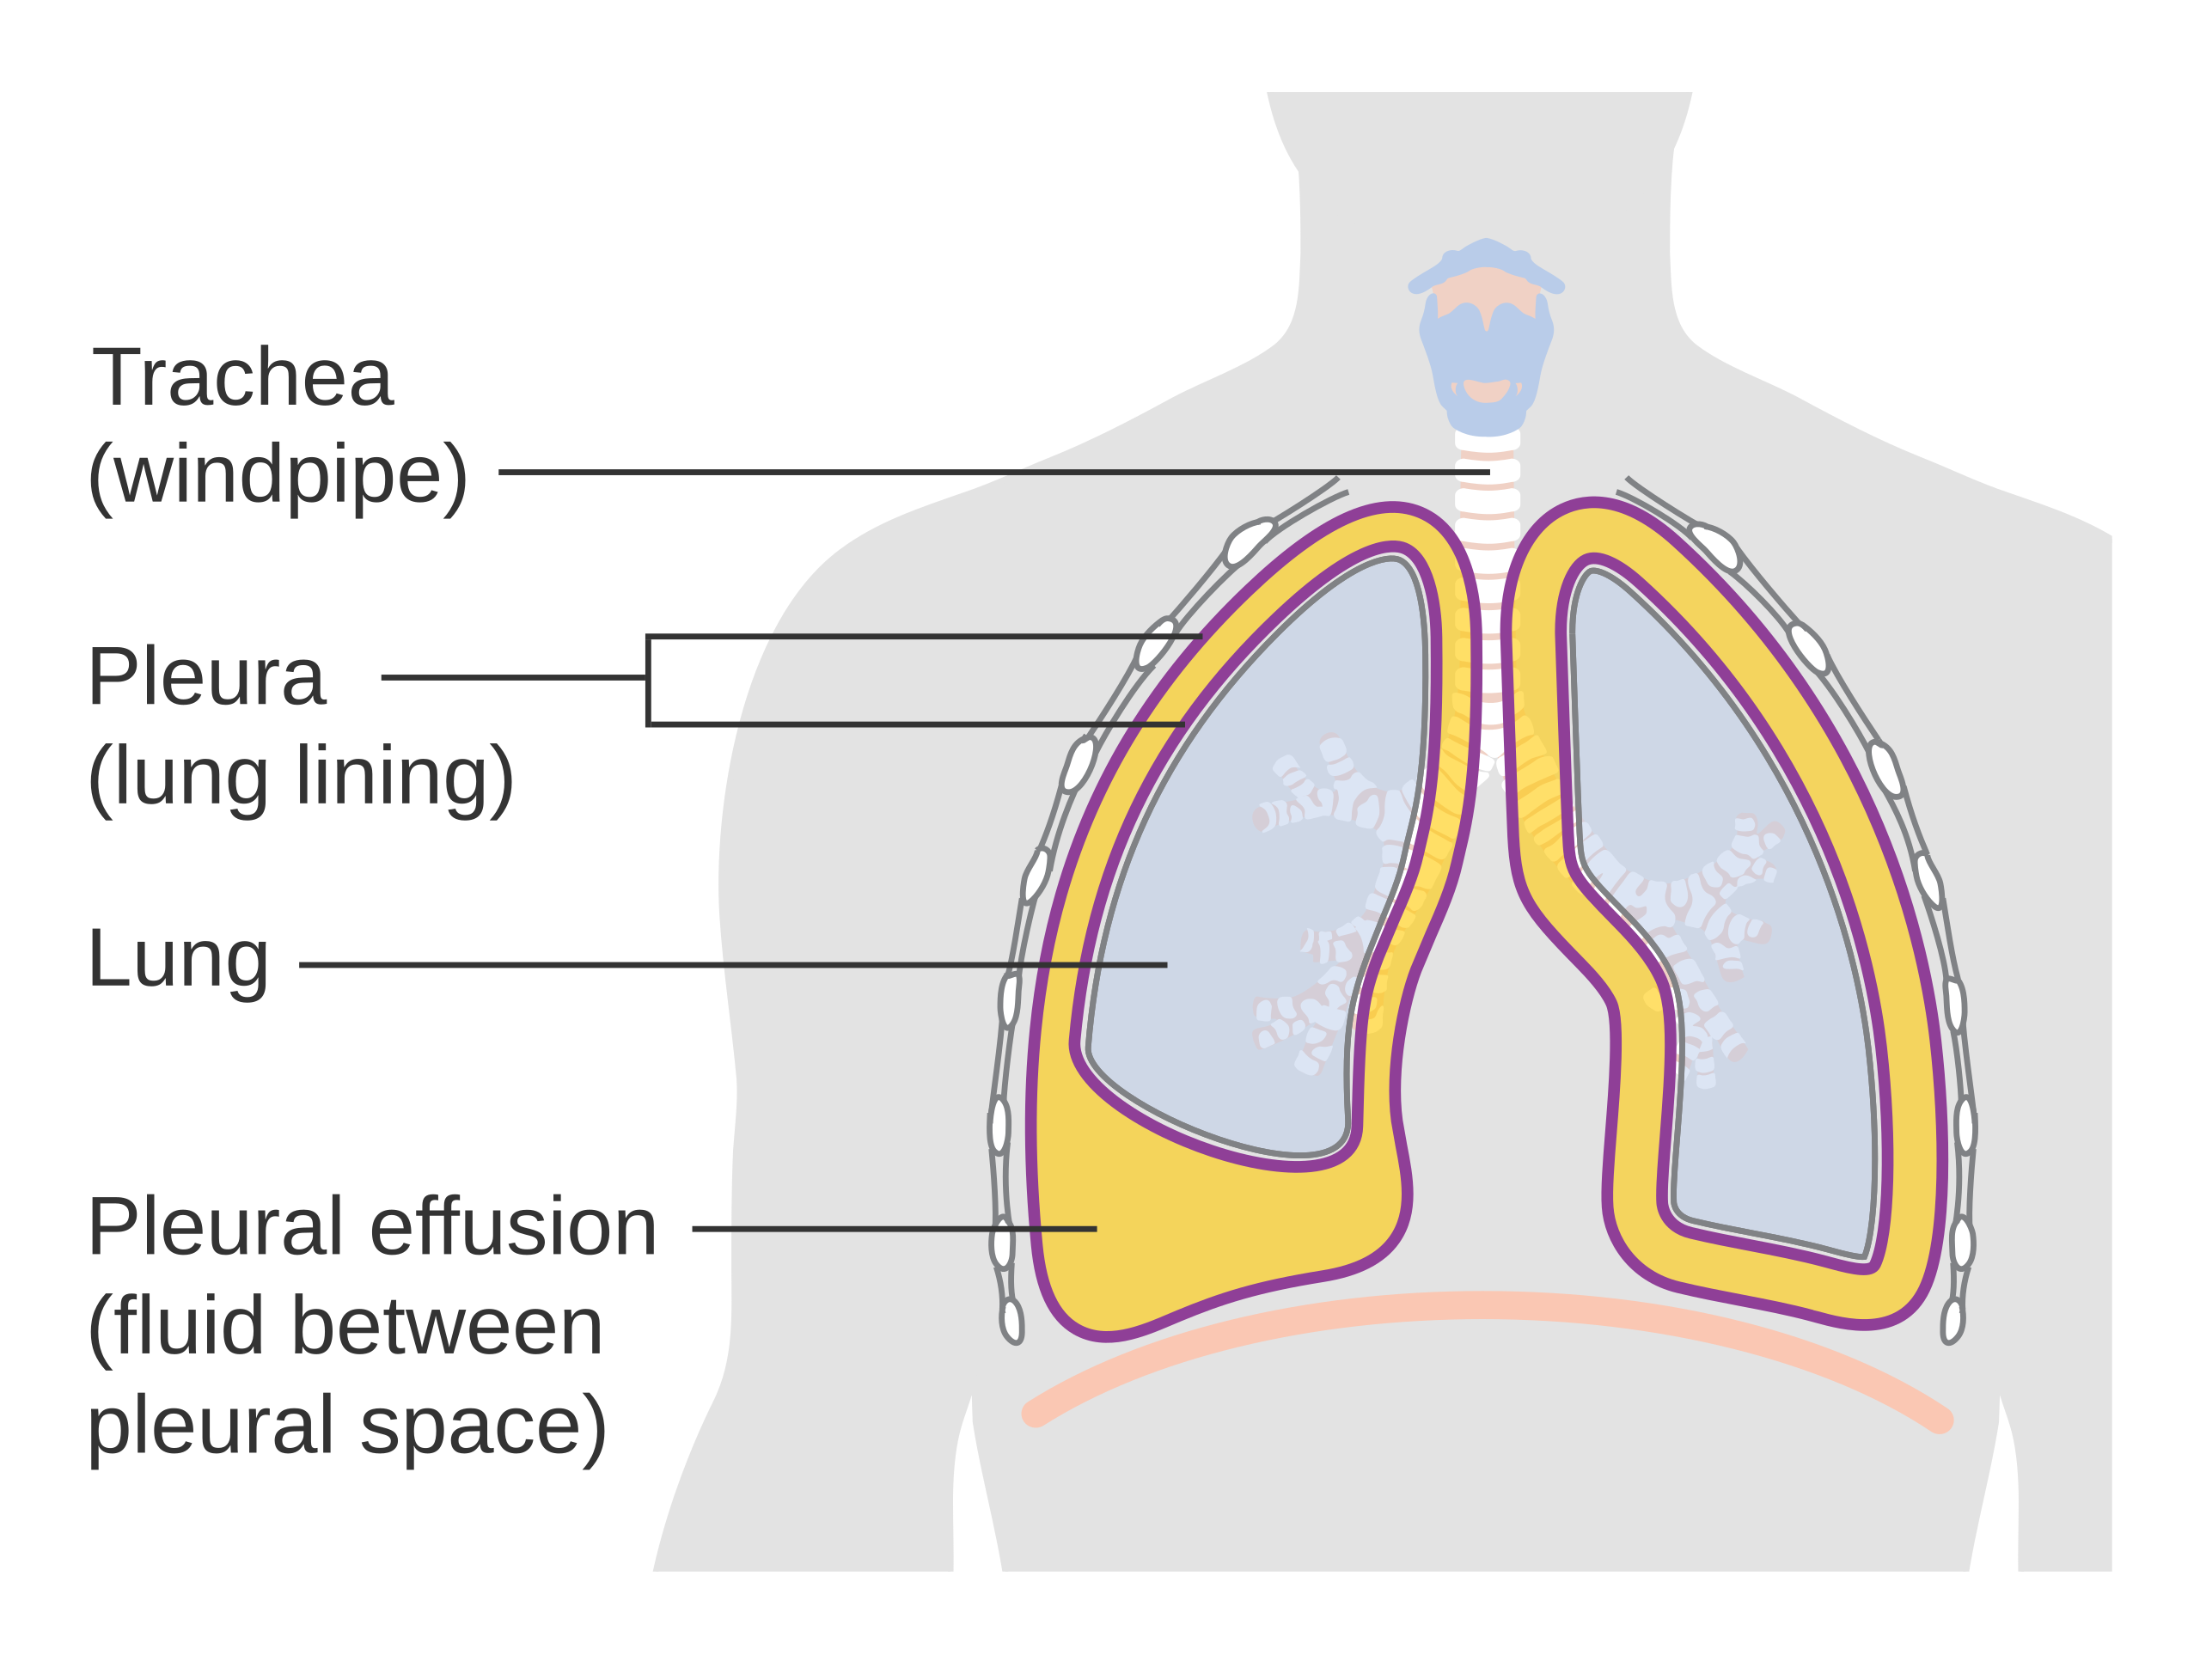
\includegraphics[keepaspectratio]{images/pleural_cavities.png}}

}

\caption{Pleural Cavities}

\end{figure}%

\section{Material \& Methods}\label{sec-data-methods}

Patients were randomly assigned to two groups: the experimental group,
which underwent median sternotomy with lungs down 10 second and two
thorax compression, and the control group without this maneuver. The
primary outcome was the incidence of pleural cavity opening given two
operators, hospital mortality. Secondary outcomes included length of
hospital stay and postoperative pain from drenages. The data was
collected from a single center and included demographic information,
surgical details, and postoperative outcomes. The data was analyzed
using statistical software to compare the outcomes between the two
groups.

\subsection{Statistical Inference}\label{statistical-inference}

All data was collected prospectively by multiple operators in a shared
single file with version control. The all manuscript was written using
Quarto Manuscript writing system with R programming incorporated. The
article is published using the github pages on authors personal page.
All the code and relevant data is available on
\href{https://github.com/raffdoc/manuscript-template}{github page}.

\section{Results}\label{results}

There were 1 (2.272727\%) patient with hospital mortality in the control
group and and none in experimental group (p = 0.32). The mean age of
patients in the experimental group was 67.9 \(\pm\) 5.6 years, while in
the control group it was 69.6 \(\pm\) 6.0 years (p = 0.18). The body
mass index (BMI) was also compared between the two groups, with a mean
BMI of 31.0 \(\pm\) 6.0 in the experimental group and 30.8 \(\pm\) 6.9
in the control group Figure~\ref{fig-bmi}. The results showed that the
experimental group had a lower incidence of pleural cavity opening
compared to the control group Figure~\ref{fig-pl-open}. The length of
hospital stay was also shorter in the experimental group, indicating a
potential benefit of the new approach.

\section{Conclusion}\label{conclusion}

The results of this study suggest that the new approach to median
sternotomy with lungs down 10 second and two thorax compression may
reduce the incidence of pleural cavity opening and improve postoperative
outcomes. Further studies with larger cohort and wider patients'
population group are needed to confirm these findings and evaluate the
long-term effects of this technique.

\section{Figures}\label{figures}

\phantomsection\label{cell-fig-pl-open}
\begin{figure}[H]

\centering{

\pandocbounded{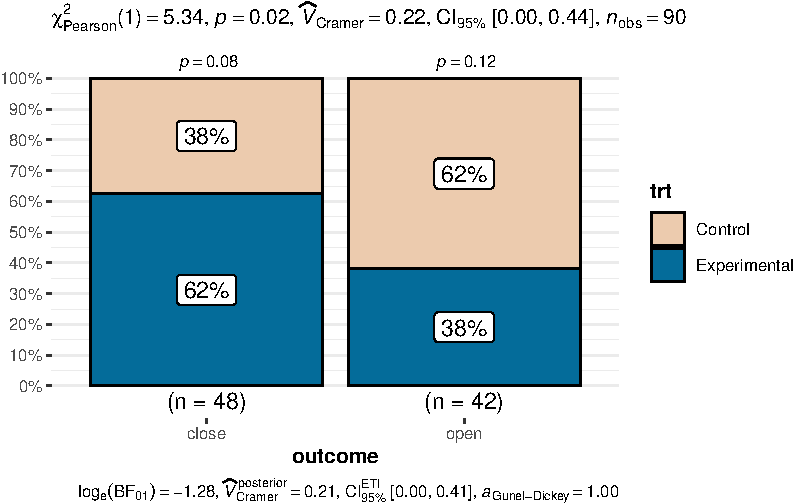
\includegraphics[keepaspectratio]{index_files/figure-pdf/fig-pl-open-1.pdf}}

}

\caption{\label{fig-pl-open}Pleural cavity opening}

\end{figure}%

\textsubscript{Source:
\href{https://raffdoc.github.io/manuscript-template/index-preview.html}{Article
Notebook}}

\phantomsection\label{cell-fig-bmi}
\begin{figure}[H]

\centering{

\pandocbounded{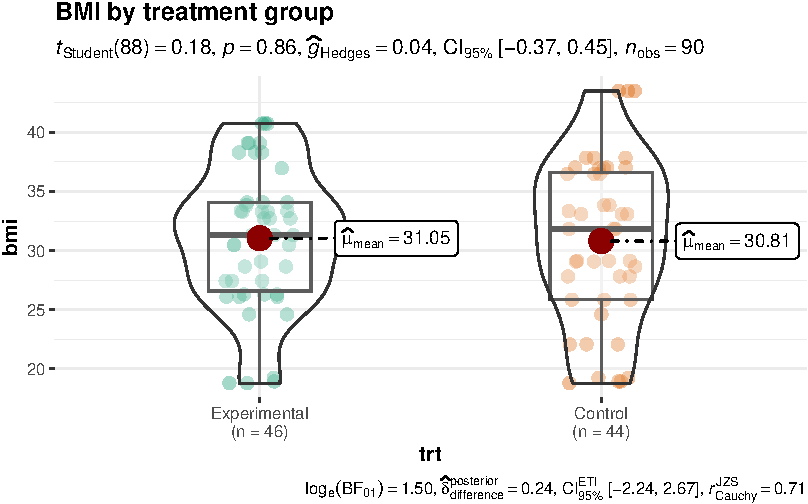
\includegraphics[keepaspectratio]{index_files/figure-pdf/fig-bmi-1.pdf}}

}

\caption{\label{fig-bmi}BMI by treatment group}

\end{figure}%

\textsubscript{Source:
\href{https://raffdoc.github.io/manuscript-template/index-preview.html}{Article
Notebook}}

\section{Tables}\label{tables}

\begin{table}

\caption{\label{tbl-demo}Demographics of the first stage}

\centering{

\fontsize{12.0pt}{14.4pt}\selectfont
\begin{tabular*}{\linewidth}{@{\extracolsep{\fill}}lcccc}
\toprule
\textbf{Characteristic} & \textbf{Overall}  N = 90\textsuperscript{\textit{1}} & \textbf{Experimental}  N = 46\textsuperscript{\textit{1}} & \textbf{Control}  N = 44\textsuperscript{\textit{1}} & \textbf{p-value}\textsuperscript{\textit{2}} \\ 
\midrule\addlinespace[2.5pt]
Pleural cavity opening &  &  &  & 0.021 \\ 
    close & 48 (53\%) & 30 (65\%) & 18 (41\%) &  \\ 
    open & 42 (47\%) & 16 (35\%) & 26 (59\%) &  \\ 
Body Mass Index & 31 (6) & 31 (6) & 31 (7) & 0.8 \\ 
Diabetis & 36 (40\%) & 20 (43\%) & 16 (36\%) & 0.5 \\ 
copd & 21 (23\%) & 11 (24\%) & 10 (23\%) & 0.9 \\ 
steroids & 12 (13\%) & 3 (6.5\%) & 9 (20\%) & 0.052 \\ 
hospital\_mortality & 1 (1.1\%) & 0 (0\%) & 1 (2.3\%) & 0.5 \\ 
hospital\_stay &  &  &  & 0.032 \\ 
    4 & 6 (6.7\%) & 4 (8.7\%) & 2 (4.5\%) &  \\ 
    5 & 30 (33\%) & 8 (17\%) & 22 (50\%) &  \\ 
    6 & 12 (13\%) & 8 (17\%) & 4 (9.1\%) &  \\ 
    7 & 18 (20\%) & 9 (20\%) & 9 (20\%) &  \\ 
    8 & 15 (17\%) & 10 (22\%) & 5 (11\%) &  \\ 
    9 & 6 (6.7\%) & 5 (11\%) & 1 (2.3\%) &  \\ 
    10 & 3 (3.3\%) & 2 (4.3\%) & 1 (2.3\%) &  \\ 
age & 68.7 (5.8) & 67.9 (5.6) & 69.6 (6.0) & 0.2 \\ 
sex &  &  &  & 0.033 \\ 
    female & 33 (37\%) & 12 (26\%) & 21 (48\%) &  \\ 
    male & 57 (63\%) & 34 (74\%) & 23 (52\%) &  \\ 
\bottomrule
\end{tabular*}
\begin{minipage}{\linewidth}
\textsuperscript{\textit{1}}n (\%); Mean (SD)\\
\textsuperscript{\textit{2}}Pearson's Chi-squared test; Wilcoxon rank sum test; Fisher's exact test\\
\end{minipage}

}

\end{table}%

\textsubscript{Source:
\href{https://raffdoc.github.io/manuscript-template/index-preview.html}{Article
Notebook}}

\section{Discussion}\label{discussion}

We have conducted a clinical trial to evaluate the effectiveness of a
new approach to median sternotomy in reducing the incidence of pleural
cavity opening. Other studies have shown that median sternotomy can lead
to complications such as pneumothorax and hemothorax, which can
significantly impact postoperative outcomes(Gullu et al. 2009).

The results of this study suggest that the new approach may be
beneficial in improving postoperative outcomes. There are several
limitations to this study, including the small sample size and the
single-center design.

\section{Acknowledgements}\label{acknowledgements}

This study was supported by institutional committee. The authors would
like to thank all the patients who participated in this study and the
medical staff for their support.

\section*{References}\label{references}
\addcontentsline{toc}{section}{References}

\phantomsection\label{refs}
\begin{CSLReferences}{1}{0}
\bibitem[\citeproctext]{ref-angelini1989}
Angelini, G. D., and A. C. Newby. 1989. {``The future of saphenous vein
as a coronary artery bypass conduit.''} \emph{European Heart Journal} 10
(3): 273--80.
\url{https://doi.org/10.1093/oxfordjournals.eurheartj.a059476}.

\bibitem[\citeproctext]{ref-gullu2009}
Gullu, Ahmet Umit, Abdurrahman Ekinci, Yavuz Sensoz, Mehmet Kızılay,
Sahin Senay, Ahmet Arnaz, Turkan Coruh, Mehmet Ates, and Murat Akcar.
2009. {``Preserved Pleural Integrity Provides Better Respiratory
Function and Pain Score After Coronary Surgery.''} \emph{Journal of
Cardiac Surgery} 24 (4): 374--78.
\url{https://doi.org/10.1111/j.1540-8191.2008.00734.x}.

\end{CSLReferences}




\end{document}
